%!TEX root=index.tex

\newacronym{ncdc}{NCDC}{National Climatic Data Center}
\newacronym{soi}{SOI}{Southern Oscillation Index}
\newacronym{tvs}{TVS}{National Tornado Vortex Signature}
\newacronym{mda}{MDA}{National Mesoscyclone Detection Algorithm}

\chapter{Case Study}
\section*{Tornado}
A primary carrier of property and casualty insurance would potentially be very interested in knowing the probability of tornado occurrence in geographical areas in which they have a large customer base. There are two months in the year which kick off tornado season in the United States: the warm season starting in March, and the cold season starting in November. Having accurate predictions of weekly seasonal tornado counts, months in advance, would constitute a significant business advantage over competitors. There are two specific business cases for the property carrier to focus on:
\begin{itemize}
    \item an actuary who will use the historical year-to-year probability and future counts to create overlays based on parcel level policy and claims data on a 50km x 50km geographical grid
    \item an underwriter who will use actuarial information to create the appropriate terms and rates offering for their customers that maximizes revenues at the lowest risk level
\end{itemize}
A working group, consisting of Dr. Christopher Anderson, Dr. Dan Walker, and myself, has determined that the data layer for tornado prediction should contain the following data sets [unpublished, 2013]:
\begin{itemize}
    \item 2.5 TB of \gls{merra} 3D historical \cite{mdisc}
    \item 1 MB of \gls{soi} historical archives \cite{bom}
    \item 100 MB of \gls{tvs} and \gls{mda} \cite{hdss}
    \item 1.5 TB of \gls{ncdc} historical tornado report \cite{ncdc}
\end{itemize}
All of this data is in the public domain and freely available to anyone that has the resources to store and analyze it. As mentioned in chapter one, currently CSC uses only the summary information provided by Giovanni in the \climatedge product. While Giovanni has the advantage of requiring no local computational resources, it represents the tip of the proverbial data iceberg and does not help in quantitative prediction.\\

Combinations of the data sets listed above can vary in size from a few hundred gigabytes to a few hundred terabytes just for the raw data. In order to quantitatively process this data, we need a service platform capable of performing the following operational layers:
\begin{itemize}
	\item retrieving data updates
	\item storing and indexing for optimal retrieval
	\item data discovery and analytics
	\item presenting real-time and offline results
\end{itemize}
\subsection*{Data Acquisition}
As all the data is freely available via standard HTTP requests, we simply need to put together a framework consisting of a repeatable process that polls each website for newly published data and retrieves it. If necessary, the framework can check with the data store to confirm what's new and what's not. Putting together such a framework is a relatively simple systems integration and development task and has plenty of prior art across the industry. I'd recommend the following components:
\begin{itemize}
	\item Three Linux instances to handle retrieval, monitoring, and hosting the source code repository, respectively.
	\item Jenkins for continually monitoring and notifying the success or failure of the retrieval processes (one per data set). Jenkins will also serve as the means to deploy the most recent code from the code repository onto the server handling the retrieval process. Jenkins is open source and used commonly across the industry for this purpose, resulting in an easily hirable skill set \cite{jenkins}
	\item A repeatable method, such as Cron, to check and retrieve updated data sets at well defined publication intervals. Jenkins will monitor the success or failure of the cron jobs and notify as needed.
	\item Developed code that contacts each web server and pulls down only the most recent data. If the data sets do not offer a simple means of determining what's recent, this code can query the data store so that it's aware of the last stored data. While we need unique code for each data set, the process of determining what's new and retrieving the code should be very similar across all the data sets. It's likely there will a reusable common library of functionality across each specific implementation. This development is likely to be done in a scriptable environment such as Python or Perl. The languages offer an excellent tradeoff between simplicity, flexibility, and execution speed.
\end{itemize}

\subsection*{Storing and Indexing}
Once the data has arrived on the local system, it needs to processed and inserted into the data store. This layer is the heart of any service offering. The data store must have the following characteristics:
\begin{itemize}
	\item Not inherently possess a single point of failure
	\item Horizontally scale (as linearly as possible) in storage and performance
	\item support realtime and batch analytics
\end{itemize}
There exist several technologies in the top level Apache Hadoop project, one being Cassandra\index{Cassandra}, which fulfill the requirements listed above\cite{cassandra}. There of competing technologies from commercial vendors like EMC, IBM, Intel, SAS, and Oracle, just to name a few, who have similar technologies designed to store and index vast amounts of data. Regardless of technology, within the data store implementation, we can use the following generic key-value model for storing any piece of climate data.
\begin{table}[htbp]
	\caption*{Climate Data Model}
	\centering
	\begin{tabular}{l l}
		\hline
		Key & Value \\ [0.5ex]
		%heading
		\hline
		meta-data & what the measurement represents, i.e., total precipitation or soil moisture\\
		time & time and date of measurement in UTC, i.e., YYYY-MM-DD HH:MM:SS\\
		coordinates & geographic location in latitude and longitude, i.e. -90.0 to 90.0 and -180.0 to 180.0\\
		value & measurement value, i.e. 0.000052977\\
		\hline
	\end{tabular}
\end{table}
With this simple structure and specific materialized views \index{materialized views}\cite{materialized_views}, we enable analytics based on any combination of the following searches: temporal, geospatial, or by meta-data.

\subsection*{Discovery and Analytics}
The technology behind big data storage is really only interesting to engineers. What we want are the results of the stored data analysis. For tornado prediction, the specific analytic we'd produce is a 50km x50km (based on data set granularity) geo-spatial grid of predictions of the probability of tornado occurrences expressed as a Poisson distribution[unpublished, 2013]. . This analytic would be computed twice a year in the months leading up to the tornado season in order to give the carriers enough time to react to the data. The \\

\subsection*{Presentation}

\begin{figure}[htbp]
    \centering
%    \caption*{Data flow by layer}
    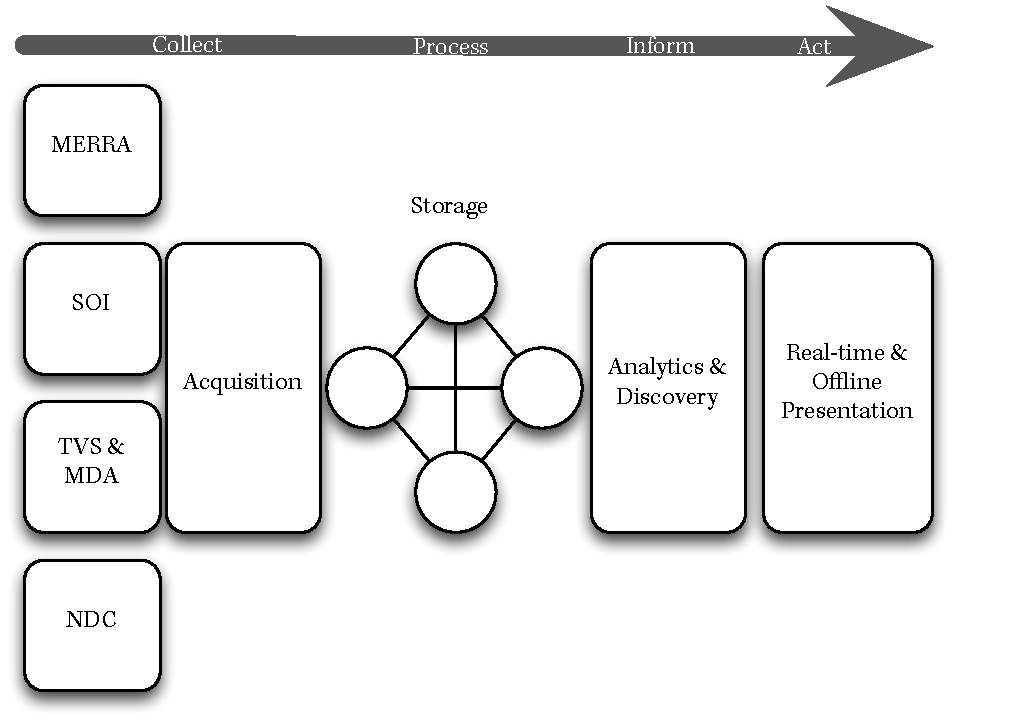
\includegraphics[scale=.9]{dataflow}
\end{figure}

%\begingroup
    % this removes the chapter title for the in-chapter bibliography
%    \renewcommand{\chapter}[2]{}% for other classes
\renewcommand\bibname{{References}}
\bibliographystyle{plain}
\bibliography{chapter2}
%\endgroup
% Review of the sources: internet, C3, books, etc plus interview with the experts
